\section{Initial Results from Pilot Study}
\label{sec:result}

To further demonstrate the viability of our approach, we present a (very) preliminary analysis of one part of the model shown in Figure~\ref{fig:model} based on our pilot data (which included only first year students, from both engineering and non-engineering majors, as shown in Table~\ref{tab:study-participants}). 

\noindent For this analysis, we focused on answering aspects of \ref{itm:rq-behavior} (the impact of daily discrimination on short-term behaviors) and \ref{itm:rq-behavior-size} (the size and length of behavior change). 

\paragraph{Analysis Approach}
We use hierarchical linear modeling (HLM) for this analysis. HLM is an extension of linear regression for units (\eg individuals, schools, communities) with correlated/common features. %We use a two-level model in which individual participants, who were repeatedly sampled over time, are clustered within themselves.
%HLM allows for flexibility in how change over time is modeled such that these models can fit discontinuous and non-linear changes. Additionally, 
HLM models do not require that individuals report the same number of observations over time and thus can handle an unequal number of observations per person and uneven spacing between observations (\cite{maas2005sufficient}).

Considering the inter-related nature of the variables and the sheer number of them, along with the small number of participants in the pilot study, the behavior features considered as outcomes must be reduced to avoid an excessive number of comparisons that increase the chance of type I error. 
\begin{wrapfigure}{l}{0.5\textwidth}
\vspace{-1.5em}
    \centering
    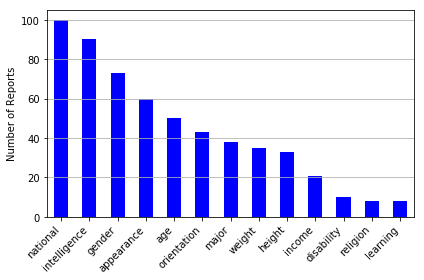
\includegraphics[width=3.3in]{img/discrimination_breakdown.png}
`    \caption[Unfair treatment type breakdown]{Breakdown of \numdiscriminationeventsfinal reports of unfair treatment by type. \textit{National}, \textit{Orientation}, and \textit{Learning} refer to ancestry or national origin, sexual orientation, and learning disability respectively. See \tbl{tab:study-surveys} for details of all categories. Participants were able to report multiple types of unfair treatment in each incident report.
}
    \label{fig:data-discrimination-breakdown}
\end{wrapfigure}
We used feature selection to reduce the size of the feature space before analysis. We select the top five metrics (when available) for each sensor for further analysis. There is much more to be said about analysis, and it is a domain in which PI Mankoff is innovating (\eg \cite{DBLP:conf/huc/EarlyFM16,DBLP:conf/chi/BanovicBCMD16,DBLP:conf/huc/KoehlerBOMD14}). Although not a focus of this proposal, we will leverage that expertise and work where useful to improve this proposed work.

\paragraph{Prevalence of daily discrimination}
The pilot study data lacked information about race-related discrimination, something corrected in the year one deployment. However it included discrimination on the basis of a range of other variables including ancestry / national origin, intelligence, and gender (the three most common) to religion, learning, and disability (the three least common, see \fig{fig:data-discrimination-breakdown}). Participants reported \numdiscriminationeventsfinal distinct incidents of unfair treatment during the pilot study. \fig{fig:data-discrimination-breakdown} shows the prevalence and breakdown of the reports of unfair treatment by category. We found that unfair treatment is more prevalent amongst women; 73\% of all reports of unfair treatment are reports from women. Contrary to our expectations, unfair treatment is equally prevalent in both engineering and non-engineering majors. 


\paragraph{\ref{itm:rq-behavior} Impact of daily discrimination on short-term behavior} We find short-term impacts of discrimination on mental health and behavior. We find that discriminatory encounters show strong (high confidence) relationships with same-day depression and frustration (\textit{p} $<.001$), but not positive affect. This is consistent with earlier reports that discrimination is more strongly associated with higher negative but not lower positive states \citep{Schmitt:2014}. Changes in depression and frustration are illustrated in Figure~\ref{fig:reeults-affect-dieoff}.  

We also find a relationship with behavior, with behaviors relating to sleep, activities, steps, and phone use all significantly different from baseline on the day of discrimination. This supports our theoretical model, which links discrimination to stress and thus predicts changes in stress-related behaviors. 

\paragraph{\ref{itm:rq-behavior-size} Size and length of shor-term behavior change}

Because of our choice to use regression modeling, we can easily quantify the impact of the changes found in ~\ref{itm:rq-behavior}. We find that people walk more (by $\sim$500 steps), have more evening calls ($\sim$1 more), interact more with their phone in the morning ($\sim$5 more interactions), and spend less time in bed ($\sim$15 minutes less). 

To model the change in impact over time, we look at exposure to discrimination on the day of (day 0) and response variables (health and behavior) on day 1, day 2 and so on, and calculate whether there is a significant difference as compared to people who report no daily discrimination.  We find that discriminatory encounters show strong (high confidence) relationships with same-day and next-day daily reports of depression and frustration. These changes in affect also translate into changes in behavior.

To relate this to behavior, we look at six of the most predictive variables found in our analysis. Our results (shown in Figure~\ref{fig:die-off}) demonstrate that most if not all of the impact found in our data occurs on  day 0 (day of the discrimination). This effect then reduces (\textit{p}-values rise) over the next two days. 
%The effect size is also stronger on the day of unfair treatment than the day after (larger $\beta$'s). After that, this distress returns to values similar to those in the control group (people who did not report unfair treatment).

\paragraph{\ref{itm:rq-short-long} Which long-term outcomes are linked to short-term behavior changes?}
Although we lack sufficient longitudinal data to fully analyze this research question (since the pilot data encompasses less than a year of the student experience), we can explore the link between behavior change and mental health. 

We use the same modeling approach to study the impact of mediating factors on the link between short term behavior change and long term outcomes. Although the immediate impact of unfair treatment fades quickly, people who report unfair treatment \textit{and} score lower on social support, report higher levels of depression at the end of the study ($\beta$ = -0.15, p-value=0.027). This is predicted by the literature  (\eg \cite{Mossakowski:2014}) and aligned with our theoretical model: having social support buffers some of the psychological distress of daily discrimination, reducing the likelihood that it will impact long-term outcomes.

\begin{figure}
     \centering

\begin{subfigure}[t]{0.49\textwidth}
%    \small
    \centering
    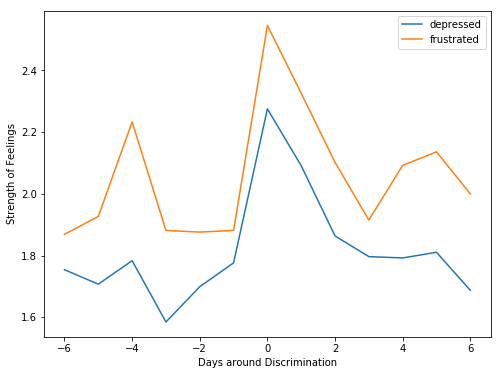
\includegraphics[width=\textwidth]{img/affect-beforeafter.png}
    \caption[Affect ratings before and after unfair treatment]{Ratings of feeling depressed and frustrated (1: not at all, 5: extremely) 6 days before and after reports of unfair treatment. Day of unfair treatment is at zero. The following days come on the right as positive numbers and the days before come on the left as negative numbers. There is a large peak on the day of the report which lasts an additional day but then more or less dies off.
    }
    \label{fig:reeults-affect-dieoff}
\end{subfigure}
\hfill
\begin{subfigure}[t]{0.49\textwidth}
    \centering
    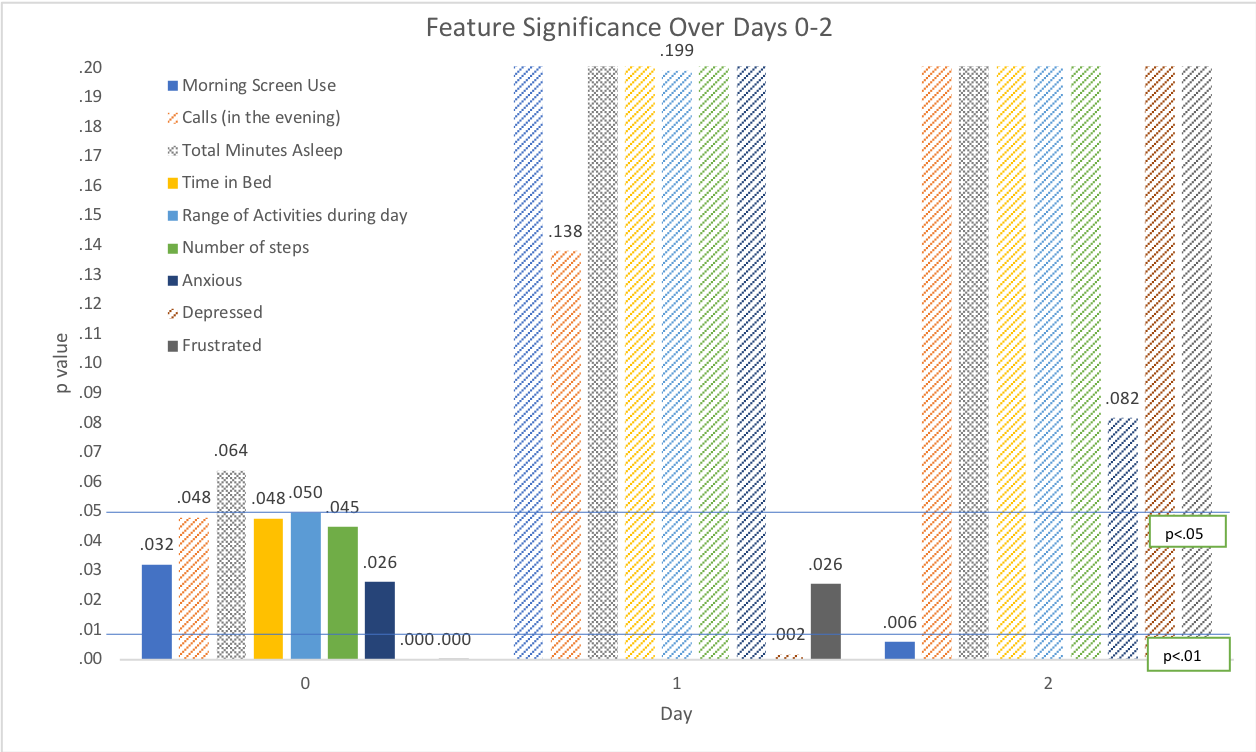
\includegraphics[width=\textwidth]{img/feature-significance}
    \caption[Feature significance over time]{Patterns of feature significance within two days of the discrimination event. The shortest bars represent the highest significance values (\eg Depressed and Frustrated on day 0; Depressed on day 1; Morning screen use on day 2) Most of short-term relations exist on the day of the event and a few on the next day.  Lines are shown at p$<.05$ and p$<.01$.\\ }
    \label{fig:die-off}
\end{subfigure}

\end{figure}


%\paragraph{Impact of microclimate and other moderators on unfair treatment:} \jen{xx to fill out. There was very old data in the proposal}
%In the chart below, the Y axis shows the percentage of engineers who were at risk on each scale in January (start of study) and June (end of study) of 2018. We choose to focus on engineers in order to compare engineers enrolled in protective micro-climates from their peers who do not share the same protective factors. These micro-climates are the Direct Admit program, in which students are directly admitted to the major and do not have to compete for admission to an engineering department; and the STARS program, which is an onboarding program for first-generation college students, and students from low-income backgrounds and high-poverty high schools in Washington; these students tend to struggle in engineering programs because they  might not be fully prepared for their prerequisite  courses. 
